\chapter{Introduction}
This chapter provides the motivation for the project and explains the background and key objectives of the thesis.
It also includes a literature review, where we outline the most important sources relevant to this work.
Finally, this chapter offers an overview of the thesis and its structure.

\begin{figure}[H]
    \centering
    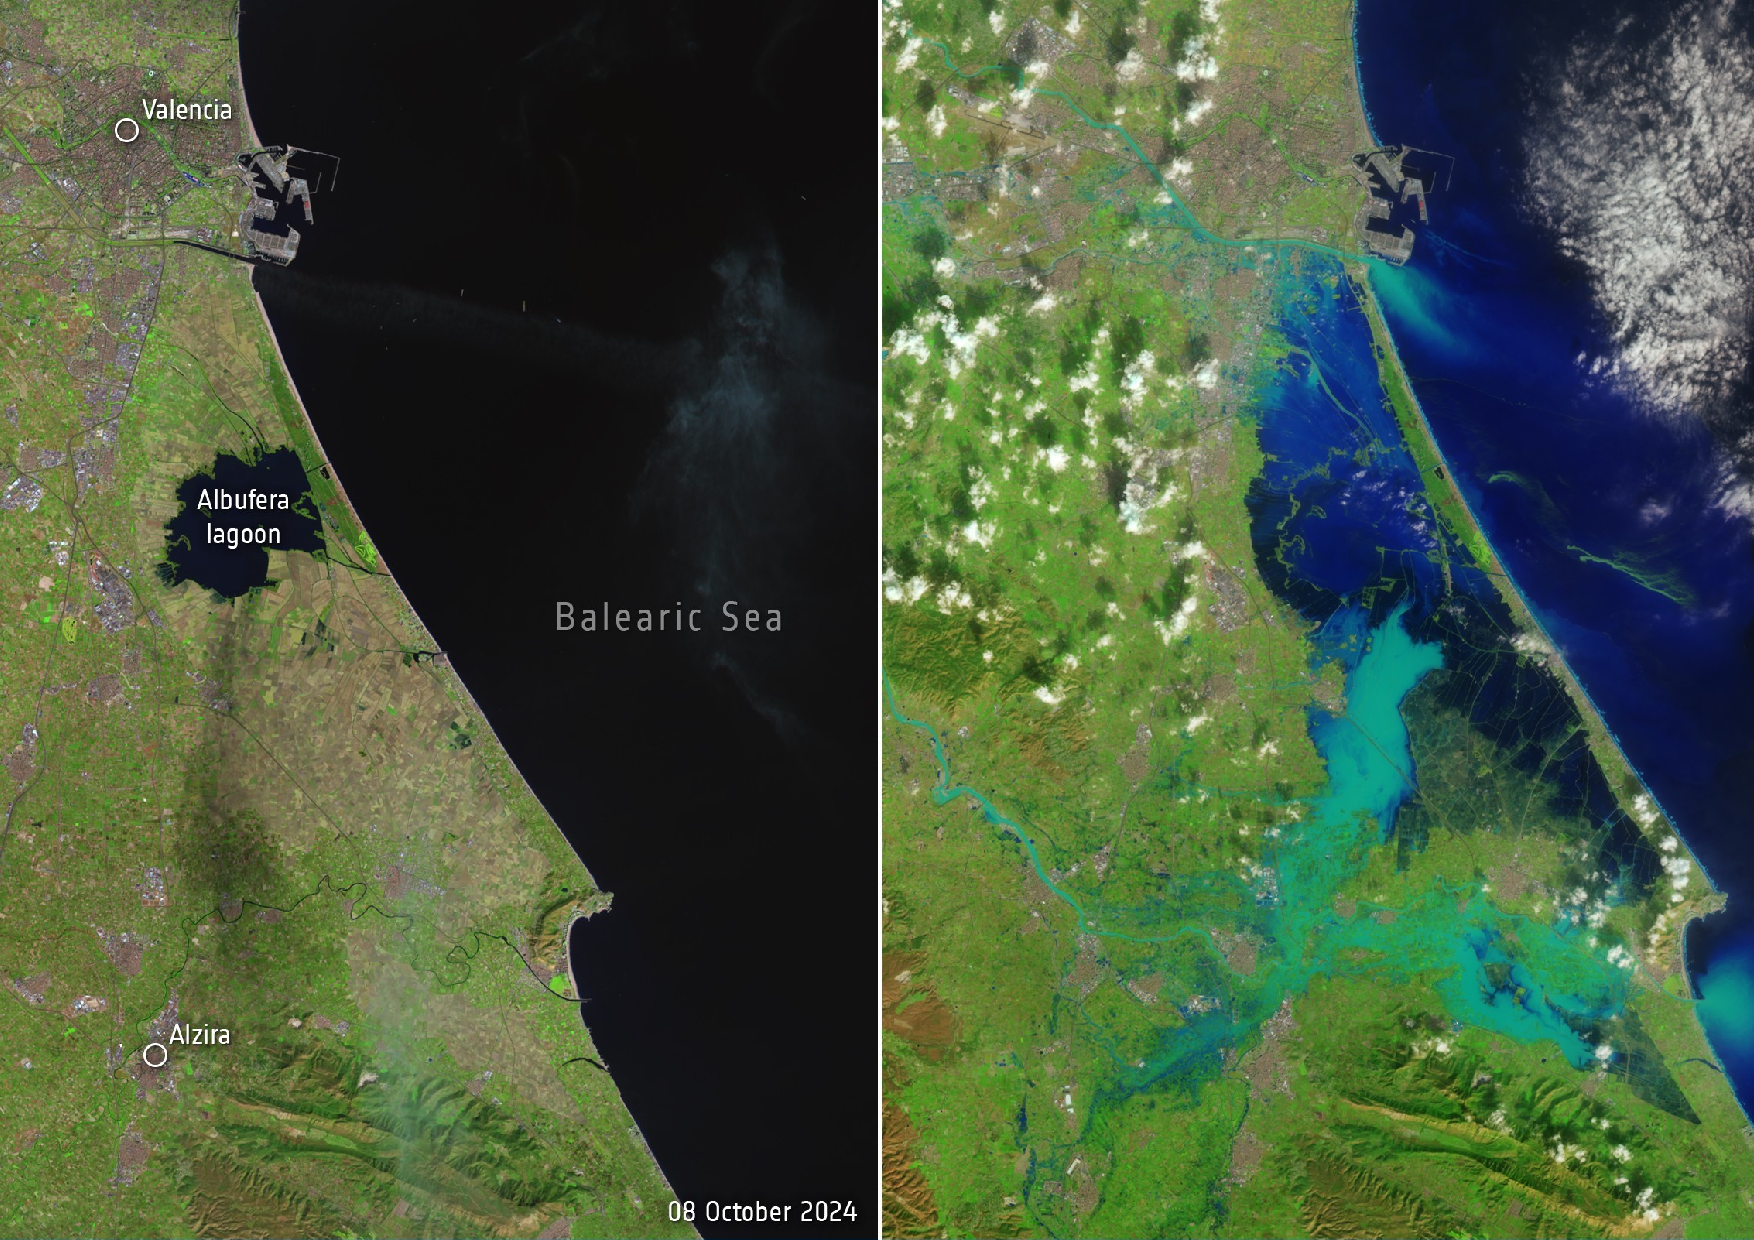
\includegraphics[width=0.7\textwidth]{C:/Users/Matteo/Shallow-Water-Equations/figs/photo_valencia.pdf}
    \caption{Before and after the floods in Valencia, Spain, October 2024.\\
            Source: \url{https://www.esa.int/ESA_Multimedia/Images/2024/10/Valencia_flood_disaster}.}
\end{figure}

\section{Motivation}
The shallow water equations (SWE) are a set of hyperbolic partial differential equations that describe the motion of a fluid in a shallow layer of water.
These equations are crucial for understanding and simulating water dynamics in shallow water regions, such as coastal areas, rivers, and flood-prone regions.
A wide range of problems can be modeled by the shallow water equations, such as flooding, tsunamis and dam break scenarios.
Recent catastrophic events, such as the floods in the Valencia region of Spain in late October 2024, highlight the urgent need for efficient tools to simulate and understand flood behavior.
On October 29, 2024, Valencia received a years worth of rain in just eight hours, leading to flash floods that devastated the area, resulting in significant loss of life and property damage~\cite{valencia_flood_disaster_esa}.

While it is impossible to prevent such disasters from occurring, a robust toolkit to solve the shallow water equations can help to create a trustworthy forecast in a sufficiently short time.
This can aid in emergency response and disaster management.
The ability to rapidly simulate flood scenarios could significantly reduce the time needed for decision-making in critical situations.
Traditional numerical methods already exist to solve the SWE, but their accuracy often comes at the cost of high computational demands.
In many cases, the run time can be too long, meaning simulations may be too slow to provide real-time insight during a flood event.
This motivates the investigation of data-driven approaches to solve the SWE fast while maintaining an acceptable level of accuracy.

By investigating data-driven methods, this project aims to determine whether they can offer a faster and more efficient way to solve the shallow water equationa compared to numerical methods.
In this work, we will derive the SWE in 1D, 2D, and spherical coordinates to model the flow of water on the Earth's surface.
We will explore the finite volume method (FVM) in 1D and 2D, a numerical technique for solving partial differential equations by dividing the domain into small control volumes and integrating the equations over these volumes.
This method is widely used in computational fluid dynamics to model fluid behavior.
We will implement the FVM and use it to solve the SWE in 1D for several problems, including the dam break problem. We will then extend this approach to 2D and solve the idealized circular dam break problem.
The FVM solvers will be validated by comparing their solutions with known test cases, as this validation is critical for generating the data needed to train the data-driven approaches.
The data-driven approaches include training a convolutional neural network (CNN) and a Fourier neural operator (FNO) to solve the shallow water equations.
The data-driven models will be trained on the FVM data and evaluated on performance metrics such as run time, accuracy, long-term prediction capabilities, grid transferability and their response to new initial conditions.
These initial conditions could include varying water heights, velocities, and other environmental factors that may change in real-world flood scenarios.
We will analyze the advantages and disadvantages of these data-driven methods and compare their run times with those of traditional numerical methods.
This comparison will allow us to assess whether data-driven approaches offer a practical solution to efficiently solving the shallow water equations, ultimately improving disaster response and flood prediction, perhaps even under varying and unforeseen initial conditions.

\section{Literature}
When working in this area it is inevitable to mention the work of E. F. Toro, who has written several books on the topic of Riemann solvers and the finite volume method, specifically for the shallow water equations.
In this project, we will use the books \textit{Shock-Capturing Methods for Free-Surface Shallow Flows}~\cite{Toro2001-Shock}, \textit{Riemann Solvers and Numerical Methods for Fluid Dynamics}~\cite{Toro2009-Riemann} and the rather new book from 2024 \textit{Computational Algorithms for Shallow Water Equations}~\cite{Toro2024} as references.
The books have been especially useful when deriving the shallow water equations as well as understanding and describing the finite volume method, inlcuding the Riemann solvers used in this project.
The course \textit{Advanced Numerical Methods for Environmental Models} at the University of Trento, has provided a good foundation for the numerical methods used in this project, both in terms of lecture notes and exercises~\cite{trento_course}.

Working with the shallow water equations in spherical coordinates, the papers \textit{Well-balanced methods for the shallow water equations in spherical coordinates} by Castro et al.~\cite{Castro2017} and \textit{Physics-informed neural networks for the shallow-water equations on the sphere} by Bihlo et al.~\cite{Bihlo2022} are references for deriving the SWE in spherical coordinates.
Additionally, the lecture notes \textit{Shallow water on a sphere} by Raymond from New Mexico Tech~\cite{Raymond} and the notes from Geophysical Fluid Dynamics Laboratory~\cite{shallow_water_gfdl} have been valuable in this derivation.
Furthermore, the papers by Gavete~\cite{Gavete_2009} and Galewsky~\cite{Galewsky_2004} also provide important insights into the spherical shallow water equations.
Implementing the FVM to solve the shallow water equations in spherical coordinates is a challenging task, as exact literature on the topic is limited.
However, some sources discussing the discontinuous Galerkin scheme~\cite{Hesthaven2008} for solving the spherical shallow water equations have been useful in this context.

The field of Fourier neural operators (FNO) is relatively new, and as a result, there is limited literature on the topic.
However, the paper \textit{Fourier Neural Operator for Parametric Partial Differential Equations}~\cite{FNO_2021}, written by several authors, is a key reference.
The paper suggests that FNOs has shown great potential in being an efficient and resolution independent operator in the emerging field of scientific machine learning to solve partial differential equations.
A key reason of their success is their ability to generalize to unseen data.
For more on the topic of scientific machine learning, consider the tech report~\cite{osti_1478744}.
In the last years the company Nvidia has done some very interesting work on the topic of FNO, and they have published several blog posts on the topic.
One of the posts consider the use of spherical Fourier neural operators (SFNO) to generate weather forecasts around the globe\cite{Nvidia2023}.
Another paper regarding SFNOs is~\cite{bonev2023-SFNO}, which generalizes FNOs on the sphere.
Convolutional neural networks (CNNs) are a well-researched area, with numerous sources available on the topic.
For this project, the sources~\cite{oshea2015introductionconvolutionalneuralnetworks} and~\cite{chollet2017comprehensive} have been particularly helpful in explaining the theoretical foundations of the methods.

\section{Thesis overview}
The rest of tge thesis is structured as follows.
In \autoref{ch:theory}, we derive the shallow water equations (SWE) in 1D, 2D, and spherical coordinates.
In \autoref{ch:fvm}, we present the finite volume method (FVM) used to solve the shallow water equations, including the Riemann problem and the numerical fluxes essential for the FVM.
These chapters form the theoretical and methodological foundation for the numerical methods employed in this project, leading into the discussion of data-driven methods.

In \autoref{ch:FNO+NN}, we introduce the concepts of convolutional neural networks (CNNs) and Fourier neural operators (FNOs), explaining how these methods can be applied to solve the shallow water equations.
In \autoref{ch:method}, we describe the process of generating the data required for the data-driven methods, as we produce all the data used in this project ourselves.

Chapter~\ref{ch:numerical_results} focuses on the numerical results for the 1D and 2D SWE using the FVM.
To validate these results, we compare the FVM outputs with test cases from the literature. Validation is crucial since the data-driven models are trained on the FVM data.
In \autoref{ch:data-driven-results}, we present the results for the shallow water equations using the data-driven models.
We analyze the outcomes, discuss the performance of the data-driven models, and compare them to the numerical results.

Finally, in \autoref{ch:discussion}, we discuss the findings, and in \autoref{ch:conclusion}, we conclude the thesis and propose directions for future work.


